% Frequency Adaptation -- 국문 초안. lualatex로 빌드.
% 최종 제출본은 SRMv2의 egPublStyle-cgf 템플릿으로 옮길 것.
\documentclass[10pt,twocolumn,a4paper]{article}
\usepackage[margin=2cm,columnsep=6mm]{geometry}
% luatexja is not installed here; plain fontspec with a Korean face is enough
% because Korean separates words with spaces, so line breaking works.
\usepackage{fontspec}
% UnBatang, not NanumMyeongjo: Nanum lacks Latin-1 diacritics, so bibliography
% author names came out as "M\u{}ller" and "B\u{}rn" with tofu boxes.
\setmainfont{UnBatang}
\setsansfont{UnDotum}
\newfontfamily\latinfont{DejaVu Serif}
\usepackage{graphicx,booktabs,amsmath,amssymb,xcolor}
\usepackage[hidelinks]{hyperref}
\usepackage{caption}
\captionsetup{font=small,labelfont=bf}
\setlength{\parskip}{0pt}
\usepackage[numbers,sort&compress]{natbib}
\usepackage{tikz}
\usetikzlibrary{positioning,calc}
\usepackage{pgfplots}
\pgfplotsset{compat=1.18}
\pgfplotsset{
  draft/.style={
    width=\columnwidth, height=41mm,
    axis lines=left, axis line style={line width=0.4pt},
    tick align=outside, tick style={line width=0.4pt, black},
    ymajorgrids, grid style={black!12, line width=0.3pt},
    label style={font=\scriptsize}, tick label style={font=\scriptsize},
    legend style={font=\scriptsize, draw=none, fill=none, cells={anchor=west},
                  inner sep=1pt},
    every axis plot/.append style={line width=0.7pt, mark size=1.7pt},
  }}
% generated by scripts/paper_numbers.py -- do not edit
\newcommand{\baseCannyClip}{30.34}
\newcommand{\baseCannyEdge}{0.6854}
\newcommand{\baseCannyFid}{71.92}
\newcommand{\baseCannyLpips}{0.5294}
\newcommand{\baseHedClip}{29.16}
\newcommand{\baseHedEdge}{0.5733}
\newcommand{\baseHedFid}{118.98}
\newcommand{\baseHedLpips}{0.6548}
\newcommand{\baseParams}{361,279,120}
\newcommand{\clipMainFiveZero}{29.78}
\newcommand{\clipMainOneHundred}{30.30}
\newcommand{\clipMainOneZero}{29.53}
\newcommand{\clipMainSevenZero}{29.92}
\newcommand{\clipMainThreeZero}{29.73}
\newcommand{\clipMainTwoZero}{29.47}
\newcommand{\clipMainZeroFive}{29.41}
\newcommand{\clipMainZero}{29.54}
\newcommand{\divHalfScale}{0.6061}
\newcommand{\divMainFiveZero}{0.4100}
\newcommand{\divMainOneHundred}{0.5066}
\newcommand{\divMainOneZero}{0.3414}
\newcommand{\divMainSevenZero}{0.4334}
\newcommand{\divMainThreeZero}{0.3794}
\newcommand{\divMainTwoZero}{0.3719}
\newcommand{\divMainZeroFive}{0.3126}
\newcommand{\divMainZero}{0.2994}
\newcommand{\divQuarterScale}{0.7752}
\newcommand{\divThreeQScale}{0.4171}
\newcommand{\edgeMainFiveZero}{0.6225}
\newcommand{\edgeMainOneHundred}{0.4724}
\newcommand{\edgeMainOneZero}{0.7439}
\newcommand{\edgeMainSevenZero}{0.5788}
\newcommand{\edgeMainThreeZero}{0.6878}
\newcommand{\edgeMainTwoZero}{0.7113}
\newcommand{\edgeMainZeroFive}{0.7796}
\newcommand{\edgeMainZero}{0.7776}
\newcommand{\fidEa}{56.39}
\newcommand{\fidEbase}{76.25}
\newcommand{\fidEcapb}{52.84}
\newcommand{\fidEcap}{53.17}
\newcommand{\fidEgate}{65.71}
\newcommand{\fidEres}{86.84}
\newcommand{\fidEwin}{58.51}
\newcommand{\fidHalfScale}{76.46}
\newcommand{\fidMainFiveZero}{53.97}
\newcommand{\fidMainOneHundred}{57.40}
\newcommand{\fidMainOneZero}{54.68}
\newcommand{\fidMainSevenZero}{53.69}
\newcommand{\fidMainThreeZero}{52.77}
\newcommand{\fidMainTwoZero}{53.45}
\newcommand{\fidMainZeroFive}{51.58}
\newcommand{\fidMainZero}{50.13}
\newcommand{\fidQuarterScale}{104.95}
\newcommand{\fidThreeQScale}{58.90}
\newcommand{\lpipsMainFiveZero}{0.4418}
\newcommand{\lpipsMainOneHundred}{0.5329}
\newcommand{\lpipsMainOneZero}{0.3748}
\newcommand{\lpipsMainSevenZero}{0.4625}
\newcommand{\lpipsMainThreeZero}{0.4148}
\newcommand{\lpipsMainTwoZero}{0.4003}
\newcommand{\lpipsMainZeroFive}{0.3495}
\newcommand{\lpipsMainZero}{0.3341}
\newcommand{\nTest}{3,500}
\newcommand{\nTrain}{65,100}
\newcommand{\ourParamsRatio}{55}
\newcommand{\ourParams}{6,611,469}
\newcommand{\pathAllOffThreeZero}{0.0087}
\newcommand{\pathAllOffZero}{0.0368}
\newcommand{\pathAttnOnlyThreeZero}{0.0279}
\newcommand{\pathAttnOnlyZero}{0.2112}
\newcommand{\pathBothThreeZero}{0.2347}
\newcommand{\pathBothZero}{0.6991}
\newcommand{\pathFidAllOff}{120.50}
\newcommand{\pathFidAttnOnly}{67.07}
\newcommand{\pathFidBoth}{50.13}
\newcommand{\pathFidSkipOnly}{65.12}
\newcommand{\pathSkipOnlyThreeZero}{0.1499}
\newcommand{\pathSkipOnlyZero}{0.5370}
\newcommand{\scEaOneZero}{0.0772}
\newcommand{\scEaThreeZero}{0.0314}
\newcommand{\scEaZeroFive}{0.1485}
\newcommand{\scEbaseOneZero}{0.0147}
\newcommand{\scEbaseThreeZero}{0.0172}
\newcommand{\scEbaseZeroFive}{0.0234}
\newcommand{\scEcapOneZero}{0.1882}
\newcommand{\scEcapThreeZero}{0.0739}
\newcommand{\scEcapZeroFive}{0.2826}
\newcommand{\scEcapbOneZero}{0.2158}
\newcommand{\scEcapbThreeZero}{0.0816}
\newcommand{\scEcapbZeroFive}{0.2986}
\newcommand{\scEgateOneZero}{0.0177}
\newcommand{\scEgateThreeZero}{0.0198}
\newcommand{\scEgateZeroFive}{0.0303}
\newcommand{\scEresOneZero}{0.0171}
\newcommand{\scEresThreeZero}{0.0291}
\newcommand{\scEresZeroFive}{0.0271}
\newcommand{\scEwinOneZero}{0.0218}
\newcommand{\scEwinThreeZero}{0.0255}
\newcommand{\scEwinZeroFive}{0.0359}
\newcommand{\scHalfScale}{0.2146}
\newcommand{\scMainFiveZero}{0.1259}
\newcommand{\scMainOneHundred}{0.0010}
\newcommand{\scMainOneZero}{0.6211}
\newcommand{\scMainSevenZero}{0.1110}
\newcommand{\scMainThreeZero}{0.2347}
\newcommand{\scMainTwoZero}{0.4019}
\newcommand{\scMainZeroFive}{0.7469}
\newcommand{\scMainZero}{0.6991}
\newcommand{\scQuarterScale}{0.0408}
\newcommand{\scThreeQScale}{0.4893}
\newcommand{\seedMeanFiveZero}{0.1304}
\newcommand{\seedMeanOneZero}{0.6245}
\newcommand{\seedMeanSevenZero}{0.1261}
\newcommand{\seedMeanThreeZero}{0.2318}
\newcommand{\seedMeanTwoZero}{0.4036}
\newcommand{\seedMeanZeroFive}{0.7479}
\newcommand{\seedStdFiveZero}{0.0093}
\newcommand{\seedStdOneZero}{0.0059}
\newcommand{\seedStdSevenZero}{0.0186}
\newcommand{\seedStdThreeZero}{0.0106}
\newcommand{\seedStdTwoZero}{0.0098}
\newcommand{\seedStdZeroFive}{0.0015}
\newcommand{\semMainFiveZero}{0.0047}
\newcommand{\semMainOneHundred}{0.0006}
\newcommand{\semMainOneZero}{0.0035}
\newcommand{\semMainSevenZero}{0.0047}
\newcommand{\semMainThreeZero}{0.0041}
\newcommand{\semMainTwoZero}{0.0037}
\newcommand{\semMainZeroFive}{0.0030}
\newcommand{\semMainZero}{0.0070}
\newcommand{\sketchFaceClip}{23.43}
\newcommand{\sketchFaceN}{40}
\newcommand{\sketchFaceSC}{0.5484}
\newcommand{\sketchSceneClip}{22.63}
\newcommand{\sketchSceneFid}{285.91}
\newcommand{\sketchSceneN}{500}
\newcommand{\sketchSceneSC}{0.1714}
\newcommand{\specFiveZero}{0.1211}
\newcommand{\specOneZero}{0.7049}
\newcommand{\specSevenZero}{0.1287}
\newcommand{\specThreeZero}{0.1214}
\newcommand{\specZFiveZero}{-0.7}
\newcommand{\specZOneZero}{+17.5}
\newcommand{\specZSevenZero}{+2.6}
\newcommand{\specZThreeZero}{-19.0}
\newcommand{\vaeNativeOneZero}{0.8562}
\newcommand{\vaeNativeSevenZero}{0.0700}
\newcommand{\vaeNativeThreeZero}{0.5773}
\newcommand{\vaeUpOneZero}{0.9599}
\newcommand{\vaeUpSevenZero}{0.1321}
\newcommand{\vaeUpThreeZero}{0.7978}


\title{\vspace{-1.5em}\bfseries 구조 조건부 확산 모델을 위한 주파수 다이얼}
\author{익명 제출}
\date{}

\begin{document}
\maketitle

\begin{abstract}
\noindent
구조 조건부 확산 어댑터는 하나의 동작점에서 학습된다. Canny 엣지, 깊이 맵,
스케치 --- 각각은 출력이 조건을 얼마나 따를지를 고정하고, 그 균형을 옮기려면
다시 학습해야 한다. 우리는 조건의 정보량을 무작위화해 어댑터 하나를 학습한다.
차단 반경 $r$을 샘플마다 뽑는 고주파 통과 필터를 쓰고, 추론 시 $r$을 다이얼로
되읽는다. FFHQ-512에서 구조 순응도는 $r{=}0.05$의 \scMainZeroFive{}에서
$r{=}0.7$의 \scMainSevenZero{}까지 내려가고 표본 다양성은 \divMainZeroFive{}에서
\divMainSevenZero{}까지 올라가며, FID는 전 구간에서 \fidMainThreeZero{}와
\fidMainOneHundred{} 사이에 머문다. 대신 어댑터 세기를 줄이면 같은 구조 순응도에
도달하는 데 FID를 최대 \fidQuarterScale{}까지 쓴다. 주파수 다이얼의
\fidMainFiveZero{}와 비교하면 두 손잡이는 대체재가 아니다.

구현 과정에서 두 가지를 발견했다. 냉동 SD VAE는 어댑터가 읽기 전에 고주파 조건을
파괴한다. 인코딩--디코딩 왕복 후 남는 조건은 $r{=}0.3$에서 \vaeNativeThreeZero{},
$r{=}0.7$에서 \vaeNativeSevenZero{}에 불과하다. 그리고 주입 위치가 용량을 압도한다.
디코더 스킵 연결에 얹은 잔차가 구조 신호의 \pathSkipOnlyZero{}를 나르는 반면
교차 어텐션 주입은 \pathAttnOnlyZero{}에 그치고, 어댑터 폭을 네 배로 늘려도
그보다 훨씬 적게 얻는다. 학습 파라미터는 \ourParams{}개로 ControlNet의
\ourParamsRatio{}분의 1이다.
\end{abstract}

\section{서론}

ControlNet~\cite{zhang2023adding}과 그 후속 연구들~\cite{mou2023adapter,zhao2023controlnet,qin2023unicontrol,li2024controlnet}은 조건부 제어를 풀고 그대로 굳혔다. Canny 엣지로
학습한 어댑터는 Canny 엣지를 따르고, 깊이로 학습한 어댑터는 깊이를 따른다.
얼마나 따를지는 학습된 가중치의 성질이므로, 같은 스케치를 더 느슨하게 반영하고
싶은 작가는 다른 체크포인트를 고르거나 가진 것이 학습된 대로 받아들여야 한다.

우리는 모델이 얼마나 귀 기울이는지가 아니라 조건 자체를 바꾼다. 조건은 정규화된
차단 반경 $r$의 방사형 고주파 통과 필터를 거친 이미지다. $r{=}0$에서 모델은
회색조 이미지를 받고 과제는 색복원이 된다. $r$이 커질수록 필터가 스펙트럼을 더
많이 제거해 $r{=}1$에서는 거의 남지 않는다. FFHQ에서 실측하면 차단 반경 $0.05$만
되어도 스펙트럼 에너지의 97.5\,\%가 사라진다. 학습은 $r$을 샘플마다 뽑으므로
가중치 하나가 전 구간을 보고, $r$은 추론 시 파라미터가 된다.

기여는 다음과 같다.

\begin{itemize}\itemsep2pt
\item 제어 다이얼. 어댑터 하나가 구조 순응도 \scMainZeroFive{}에서
      \scMainSevenZero{}까지를 담당하며 FID는 \fidMainThreeZero{}와
      \fidMainOneHundred{} 사이로 평평하다 (\ref{sec:dial}절).
\item 이 다이얼이 어댑터 세기를 다시 스케일한 것이 아니라는 근거. 구조 순응도를
      맞추면 세기 손잡이는 FID \fidQuarterScale{}을 쓰고 주파수 손잡이는
      \fidMainFiveZero{}를 쓴다 (\ref{sec:strength}절).
\item 고주파 조건이 냉동 VAE를 얼마나 통과하는지에 대한 측정. 잠재 공간 조건화가
      희소한 구조에서 실패하는 이유를 설명한다 (\ref{sec:vae}절).
\item 주입 위치가 어댑터 용량이나 수용 영역보다 중요함을 보이는 통제 비교
      (\ref{sec:where}절).
\end{itemize}

\section{관련 연구}

\paragraph{조건부 제어.} 텍스트-이미지 확산 모델
\cite{ho2020denoising,song2020denoising,rombach2021high,nichol2021glide,saharia2022photorealistic}은
ControlNet~\cite{zhang2023adding}으로 공간 제어가 가능해졌다. 인코더를 복제하고
0 합성곱으로 잔차를 주입하는 방식이다. T2I-Adapter~\cite{mou2023adapter}는 작은
특징 추출기로 같은 일을 하고, IP-Adapter~\cite{ye2023adapter}는 이미지 프롬프트를
위한 분리형 교차 어텐션을 더하며, GLIGEN~\cite{li2023gligen}은 박스로 생성을
접지한다. Uni-ControlNet~\cite{zhao2023controlnet}과
UniControl~\cite{qin2023unicontrol}은 여러 조건 유형을 한 모델에 담고,
ControlNet++~\cite{li2024controlnet}는 생성된 이미지에서 일관성 루프를 닫는다.
이들 모두 조건 유형을 고정하고, 그와 함께 출력이 얼마나 따를지도 고정한다.
동작점이 학습된 가중치의 성질이 되는 것이다. 우리의 차단 반경은 가중치 하나에서
추론 시 그 점을 옮긴다.

\paragraph{트랜스포머 백본에서의 효율적 제어.} 백본이 UNet에서 확산
트랜스포머~\cite{peebles2022scalable,esser2024scaling}로 옮겨가면서 제어도 복제
인코더에서 경량 모듈로 이동했다. ControlNeXt~\cite{peng2024controlnext}는 병렬
분기를 없애고, OminiControl~\cite{tan2024ominicontrol}은 백본 자체를 조건
처리기로 재사용하며, EasyControl~\cite{zhang2025easycontrol}과
NanoControl~\cite{liu2025nanocontrol}은 LoRA~\cite{hu2021lora} 계열 모듈로 훨씬
적은 파라미터에서 조건을 주입한다. 조건이 어디로 들어가야 하는지도 최근 연구
대상이다. Laytrol~\cite{huang2025laytrol}은 레이아웃 제어에서 사전학습 지식
보존을, PixelControl~\cite{lin2026pixelcontrol}은 조건 충실도를,
\citet{zhou2026rethinking}은 다중 조건 DiT의 중복 어텐션 제거를 다룬다. 우리의
주입 위치 비교(\ref{sec:where}절)는 UNet 백본에서 양립하는 결론에 도달한다.
위치가 용량을 압도한다.

\paragraph{확산 모델에서의 주파수.} 주파수 분해는 확산 연구에서 대개 조건이 아니라
모델 자신의 신호에 대한 개입으로 나타난다. FreeU~\cite{si2023freeu}는 스킵과 백본
특징을 학습 없이 스펙트럼 상에서 재조정하고, FreSca~\cite{huang2025fresca}는 노이즈
예측의 주파수 대역을 스케일하며 우리처럼 에너지 기반 차단을 쓴다.
DeCo~\cite{ma2025deco}는 픽셀 공간 확산에서 주파수를 분리하고,
FeRA~\cite{yin2025fera}는 주파수 에너지로 적응을 라우팅한다.
FOCUS~\cite{tjio2025focus}는 테스트 시 적응을 위해 학습된 주파수 사전으로 역과정을
조건화한다. 취지상 가장 가까운 것은 \citet{prasain2026beyond}로, 지도-위성 합성에서
엣지 맵 대신 웨이블릿 대역으로 조건화한다. 그러나 어느 연구도 학습 중 조건의
대역폭을 무작위화해 그 대역이 추론 시 제어가 되게 하지는 않으며, 그것이 우리가
다루는 기제다.

\paragraph{구조 보존.} StructDiff~\cite{he2026structdiff}는 구조 보존형 공간 제어
생성을 목표로 하고, 스케치 조건 파이프라인은 오래전부터 엣지 맵을 구조 전달자로
써 왔다. 우리 조건은 고정된 추출기가 아니라 연속체이며, 그것이 다이얼을 가능하게
한다.

\paragraph{학습과 평가.} 분류자 없는 유도~\cite{ho2022classifier} 드롭아웃과
Min-SNR 손실 가중~\cite{hang2023efficient}으로 학습하고,
FID~\cite{heusel2017gans}를 clean-FID 프로토콜~\cite{parmar2021aliased}로,
LPIPS~\cite{zhang2018unreasonable}와 CLIP 점수~\cite{radford2021learning}를
BLIP~\cite{li2022blip} 캡션이 달린 FFHQ~\cite{karras2018style}에서 평가한다.
SDXL과 SD3~\cite{podell2023sdxl,esser2024scaling}가 다음 백본으로 자연스럽다.

\section{방법}

\paragraph{조건.} 이미지 $x$를 회색조로 바꾸고 2차원 FFT를 취한 뒤 반지름
$r \cdot \min(H,W)/2$ 원판 안의 모든 주파수를 0으로 만들고 역변환한 다음
$[0,1]$로 최소--최대 정규화한다. 정규화는 의도적이다. 필터 응답의 절대 크기를
없애 모델이 공간 통계만으로 구조 밀도를 추론하게 만든다. $r$이 존재하지 않는
손그림을 추론 시 쓸 수 있는 이유가 여기에 있다. 그림~\ref{fig:mask}는 마스크와
마스킹된 스펙트럼, 그리고 그 결과 조건을 전 구간에 걸쳐 나란히 보여준다.

% What the dial actually does, from radial_mask_numpy / high_pass_numpy in the
% repository, so the picture and the method cannot diverge.
\begin{figure*}[t]
\centering

\includegraphics[width=\textwidth]{figures/mask}
\caption{주파수 쪽에서 본 다이얼. 열은
$r = 0,\,0.05,\,0.1,\,0.2,\,0.3,\,0.5,\,0.7,\,1.0$이다. \textbf{1행:} 방사형 마스크,
검은 부분이 제거된다. \textbf{2행:} 마스킹 후 로그 크기 스펙트럼으로, 구멍이 바깥으로
커진다. \textbf{3행:} 모델이 실제로 받는 조건. \textbf{4행:} 같은 데이터를 $\pm2\sigma$로
표시해 남아 있는 내용을 드러낸 것. $r{\approx}0.2$ 위에서 조건은 평평한 회색으로 보이고
표준편차도 $r{=}0$의 0.196에서 $r{=}1$의 0.041로 떨어지지만, 4행에는 얼굴 윤곽이 남아
있고 모델은 $r{=}0.2$에서 SC \scMainTwoZero{}에 도달한다. 낮은 대비가 정보 없음을
뜻하지 않으며, 이미지별 정규화가 모델에 그것을 학습하도록 강제한다.}
\label{fig:mask}
\end{figure*}


\paragraph{조건 인코더.} 스트라이드 합성곱 스템이 $512^2$ 조건 이미지를 직접 읽어
$8\times$ 줄인다. 조건을 냉동 VAE로 인코딩하지 않는다. 이유는 \ref{sec:vae}절에 있다.

\paragraph{주입.} 인코더 특징은 UNet에 두 곳으로 들어간다. 0으로 초기화된
$1{\times}1$ 헤드가 디코더 스킵 텐서마다 잔차 하나와 중간 블록용 잔차 하나를
만들어 UNet의 기존 ControlNet 인터페이스로 더한다. 동시에 각 교차 어텐션 지점이
조건 특징의 $3{\times}3$ 창을 참조하며, 0으로 초기화된 채널별 게이트를 거친다.
두 경로 모두 초기에는 정확한 무연산이다. 둘을 끄면 네트워크가 원본
Stable Diffusion~1.5~\cite{rombach2021high}를 비트 단위로 재현하며, 모든 학습 전에 이를 검사한다.

% 저자가 직접 그린 시스템 개요. 슬라이드(images/Frequency_Adapataion.pdf 6쪽)에서
% 벡터로 내보내 잉크 경계로 잘랐다. 그림이 담지 않은 것 -- 두 번째 학습 인코더,
% 헤드 개수, 무엇이 동결인지 -- 는 캡션에 있다.
\begin{figure*}[t]
\centering
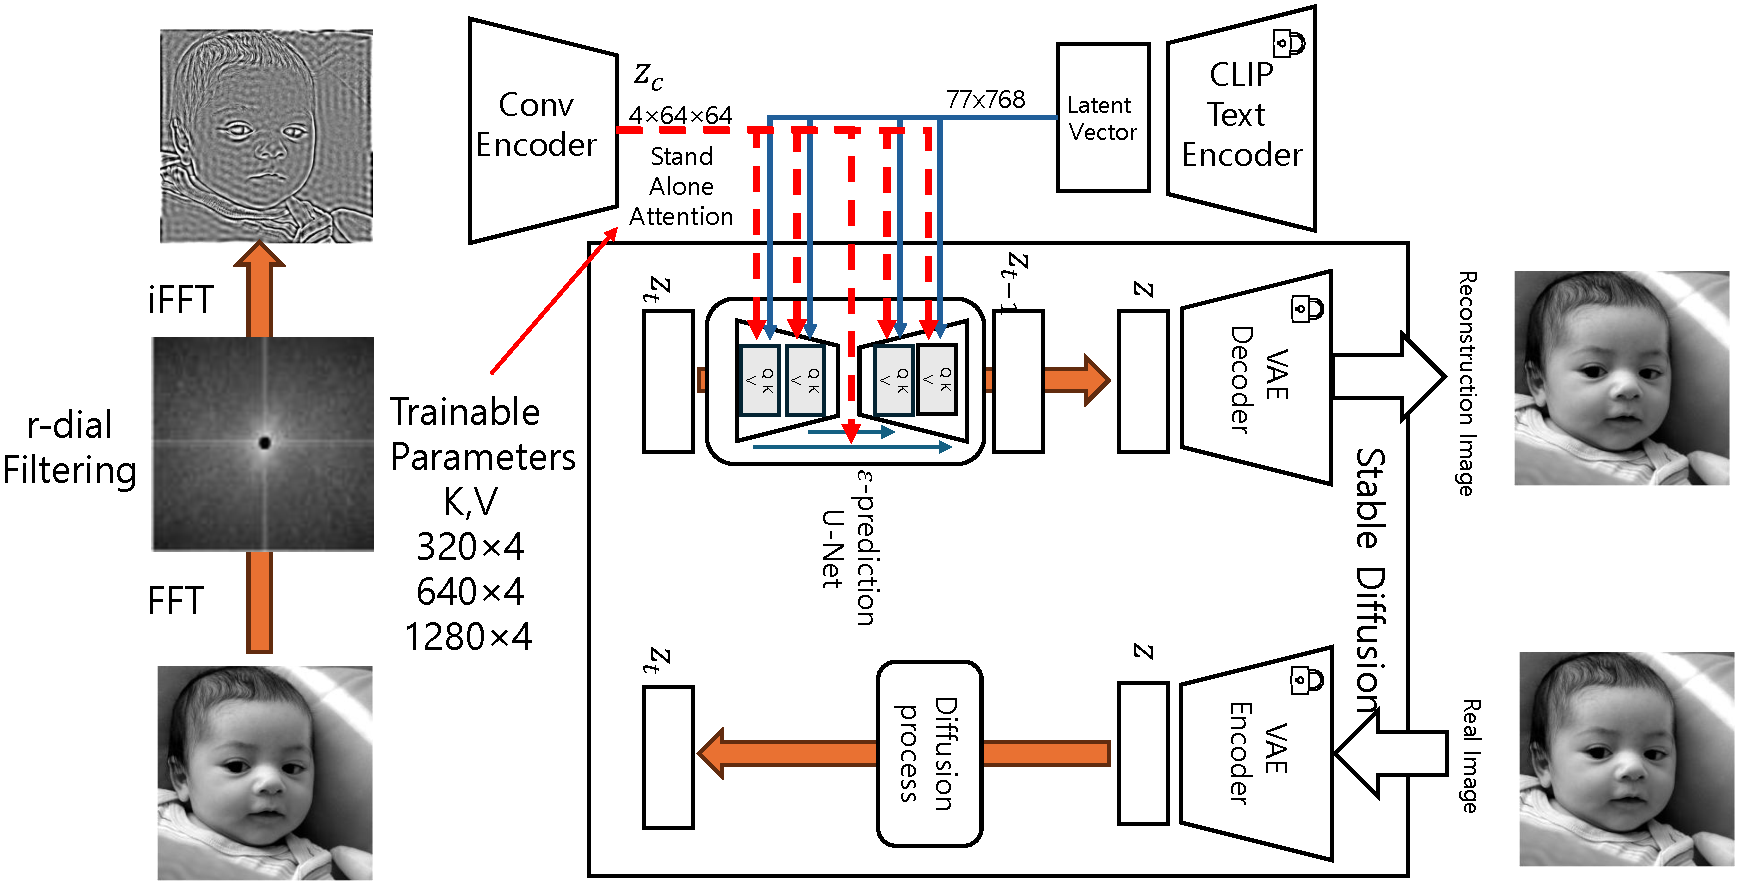
\includegraphics[width=\textwidth]{figures/pipeline}
\caption{반경 $r$의 원판을 스펙트럼에서 제거하고, 학습되는 합성곱 인코더가 그 결과를
전체 해상도로 읽어 VAE를 거치지 않고 4채널 $64{\times}64$의 조건 $z_c$를 만든다. 이는
동결 UNet의 교차 어텐션 16곳으로 들어가며, 그곳에서 학습되는 것은 $W_K$, $W_V$와
0초기화 출력 게이트뿐이고 $W_Q$와 $W_O$는 동결이다(그림~\ref{fig:sa}). 같은 조건 경로의
일부로 그려진 두 번째 학습 stem은 원본 조건을 읽어 디코더 skip 텐서 12곳과 mid block에
0초기화 잔차를 더한다. 구조의 대부분은 그 경로가 나르며, 분배는 측정된 값이다.
$r{=}0$에서 skip 경로만 켜면 SC가 \pathSkipOnlyZero{}, 어텐션만 켜면
\pathAttnOnlyZero{}다(\ref{sec:where}절). 학습은 Min-SNR 가중의 $\epsilon$ 예측이고,
동결 오토인코더를 지나는 루프는 표준 잠재 확산 그대로이며 학습되지 않는다.}
\label{fig:arch}
\end{figure*}


\paragraph{학습.} SD1.5~\cite{rombach2021high}는 냉동한다. BLIP~\cite{li2022blip} 캡션이 달린
FFHQ-512~\cite{karras2018style} \nTrain{}장에서
\ourParams{}개 파라미터를 배치 32, bf16, 12에폭, H200 한 장으로 학습한다.
$r$은 샘플마다 $[0,1]$ 균등분포에서 뽑는다.

\section{실험}

보류한 \nTest{}장에서 샘플러 50스텝, CFG 7.5, 시드 2026으로 평가한다. FID~\cite{heusel2017gans}는 clean-FID 프로토콜~\cite{parmar2021aliased}로,
LPIPS~\cite{zhang2018unreasonable}와 CLIP 점수~\cite{radford2021learning}를 함께 보고한다.
구조 순응도(SC)는 생성된 이미지에서 같은 차단 반경으로 조건을 다시 추출해 모델이 받은
조건과 상관을 낸다. 정답 이미지를 그대로 넣으면 모든 $r$에서 정확히 1.000이 나오고,
무관한 얼굴은 $r{=}0$에서 0.122, 그 위에서는 ${\approx}{-}0.02$가 나온다.

\begin{figure*}[t]
\centering

\includegraphics[width=\textwidth]{figures/dial}
\caption{시드와 캡션을 고정하고 $r$만 바꾼 결과. 왼쪽부터 참조 이미지,
$r = 0,\,0.05,\,0.1,\,0.3,\,0.5,\,0.7,\,1.0$. 배경의 인파가 옅어지고 안경테가
참조에서 멀어지며 옷 색이 분리되는 반면 신원과 자세는 남는다. 참조 이미지는
모델에 주어지지 않는다.}
\label{fig:dial}
\end{figure*}

\subsection{다이얼}
\label{sec:dial}

표~\ref{tab:main}이 동작 곡선이다. 구조 순응도는 $r{=}0.05$부터 단조 감소하고
표본 다양성은 단조 증가한다. 다이얼이 드러내야 할 균형이 그대로 나타난다. FID는 전 구간에서
\fidMainZero{}과 \fidMainOneHundred{} 사이에 머무르므로, 구간이 끝까지 쓸 만하게
유지되고 잡음으로 무너지지 않는다.

그림~\ref{fig:dial}은 시드와 캡션을 고정하고 $r$만 바꾼 것이다.
그림~\ref{fig:curve}는 곡선과, 그 아래에 두 다이얼을 같은
구조 순응도/FID 평면에 함께 놓은 것이다.

% Operating curves. Both panels read curve.dat / scale.dat, which
% scripts/paper_numbers.py writes out of results/, so a plotted point cannot
% drift from the run that produced it. Drafted to match the text: hairline
% axes, no boxes, no fills, marks a reader can count.
\begin{figure}[t]
\centering
\pgfplotsset{
  draft/.style={
    width=\columnwidth, height=41mm,
    axis lines=left, axis line style={line width=0.4pt},
    tick align=outside, tick style={line width=0.4pt, black},
    ymajorgrids, grid style={black!12, line width=0.3pt},
    label style={font=\scriptsize}, tick label style={font=\scriptsize},
    legend style={font=\scriptsize, draw=none, fill=none, cells={anchor=west},
                  inner sep=1pt},
    every axis plot/.append style={line width=0.7pt, mark size=1.7pt},
  }}
\begin{tikzpicture}
\begin{axis}[draft, xlabel={차단 반경 $r$}, ylabel={SC / 다양성 (LPIPS)},
             xmin=-0.03, xmax=1.03, ymin=0, ymax=0.8,
             legend pos=north east]
  \addplot[mark=square*, black] table[x=r, y=sc] {curve.dat};
  \addlegendentry{구조 순응도}
  \addplot[mark=o, black, densely dashed] table[x=r, y=div] {curve.dat};
  \addlegendentry{표본 다양성}
\end{axis}
\end{tikzpicture}

\vspace{2mm}

\begin{tikzpicture}
\begin{axis}[draft, height=32mm,
             xlabel={구조 순응도}, ylabel={FID},
             xmin=-0.03, xmax=0.8, ymin=45, ymax=112,
             legend columns=2,
             legend style={at={(0.5,-0.42)}, anchor=north}]
  % curve.dat의 행 순서는 r = 0, 0.05, 0.1, 0.2, 0.3, 0.5, 0.7, 1이며 1--4행이
  % 주장하는 구간이다. \thisrow{r} 표현식 필터가 pgfplots 파서를 통과하지 못해
  % 행 인덱스로 나눈다.
  \addplot[mark=square*, black, skip coords between index={0}{1}, skip coords between index={5}{8}] table[x=sc, y=fid] {curve.dat};
  \addlegendentry{차단 반경, 자기 계측기}
  \addplot[only marks, mark=square, black!45, skip coords between index={1}{5}] table[x=sc, y=fid] {curve.dat};
  \addlegendentry{차단 반경 $r > 0.3$}
  \addplot[mark=diamond*, black, densely dotted] coordinates {(\fixInstZeroFive,\fidMainZeroFive) (\fixInstOneZero,\fidMainOneZero) (\fixInstTwoZero,\fidMainTwoZero) (\fixInstThreeZero,\fidMainThreeZero)};
  \addlegendentry{차단 반경, 계측기 $r_m{=}0.1$}
  \addplot[mark=o, black, densely dashed] table[x=sc, y=fid] {scale.dat};
  \addlegendentry{무작위-$r$, $r{=}0.1$에서 스케일}
  \addplot[mark=triangle, black!55, dotted] coordinates {(\sscSCQuarter,\sscFidQuarter) (\sscSCHalf,\sscFidHalf) (\sscSCThreeQ,\sscFidThreeQ) (\sscSCOne,\sscFidOne)};
  \addlegendentry{고정-$r{=}0.1$ 어댑터, 스케일}
\end{axis}
\end{tikzpicture}
\caption{\textbf{위:} 차단 반경에 대한 구조 순응도와 표본 다양성(표~\ref{tab:main}의
값이며 SEM과 시드 sd도 거기에 있다). \textbf{아래:} 구조 순응도에 대한 FID, 점마다 FID 추정은
하나다. 채운 사각형은 $r \in [0.05, 0.3]$에서 자기 차단 반경으로 채점한 스윕, 빈 회색 사각형은
같은 스윕의 구간 밖이다. 마름모는 같은 생성물을 계측기 $r_m{=}0.1$로 다시 채점한 것이다. 원과
삼각형은 무작위-$r$ 어댑터와 고정-$r{=}0.1$ 어댑터를 $r{=}0.1$에서 스케일한 것으로, 이미
$r_m{=}0.1$을 쓴다. 그 한 계측기에서 차단 반경 $r{=}0.3$은 FID \fidMainThreeZero{}에서
\fixInstThreeZero{}에, 세기 0.50은 FID \fidHalfScale{}에서 \fixInstHalfScale{}에 이른다.
두 패널 모두 평가 출력에서 직접 그렸다.}
\label{fig:curve}
\end{figure}


\begin{table}[t]\centering\small
\begin{tabular}{lrrrrr}
\toprule
$r$ & SC & 다양성 & LPIPS & CLIP & FID \\
\midrule
0.00 & \scMainZero      & \divMainZero      & \lpipsMainZero      & \clipMainZero      & \fidMainZero \\
0.05 & \scMainZeroFive  & \divMainZeroFive  & \lpipsMainZeroFive  & \clipMainZeroFive  & \fidMainZeroFive \\
0.10 & \scMainOneZero   & \divMainOneZero   & \lpipsMainOneZero   & \clipMainOneZero   & \fidMainOneZero \\
0.20 & \scMainTwoZero   & \divMainTwoZero   & \lpipsMainTwoZero   & \clipMainTwoZero   & \fidMainTwoZero \\
0.30 & \scMainThreeZero & \divMainThreeZero & \lpipsMainThreeZero & \clipMainThreeZero & \fidMainThreeZero \\
0.50 & \scMainFiveZero  & \divMainFiveZero  & \lpipsMainFiveZero  & \clipMainFiveZero  & \fidMainFiveZero \\
0.70 & \scMainSevenZero & \divMainSevenZero & \lpipsMainSevenZero & \clipMainSevenZero & \fidMainSevenZero \\
1.00 & \scMainOneHundred& \divMainOneHundred& \lpipsMainOneHundred& \clipMainOneHundred& \fidMainOneHundred \\
\bottomrule
\end{tabular}
\caption{동작 곡선. 테스트 \nTest{}장 중 500장 샘플.}
\label{tab:main}
\end{table}

시드 2026, 2027, 2028에서 곡선은 안정적이다. $r{=}0.05$의 SC는
\seedMeanZeroFive{}\,$\pm$\,\seedStdZeroFive{}, $r{=}0.3$은
\seedMeanThreeZero{}\,$\pm$\,\seedStdThreeZero{}다.

\subsection{세기는 같은 손잡이가 아니다}
\label{sec:strength}

당연한 대안은 하나의 차단 반경으로 학습하고 추론 시 어댑터 기여를 스케일하는
것이다. 같은 체크포인트에서 $r{=}0.1$을 고정하고 두 주입 경로를 함께 스케일해
시험했다.

\begin{table}[h]\centering\small
\begin{tabular}{lrrr}
\toprule
설정 & SC & 다양성 & FID \\
\midrule
세기 0.25          & \scQuarterScale & \divQuarterScale & \fidQuarterScale \\
세기 0.50          & \scHalfScale    & \divHalfScale    & \fidHalfScale \\
세기 0.75          & \scThreeQScale  & \divThreeQScale  & \fidThreeQScale \\
\midrule
$r{=}0.3$ (우리)    & \scMainThreeZero & \divMainThreeZero & \fidMainThreeZero \\
$r{=}0.5$ (우리)    & \scMainFiveZero  & \divMainFiveZero  & \fidMainFiveZero \\
\bottomrule
\end{tabular}
\caption{세기 다이얼과 주파수 다이얼. 같은 SC에서 읽으면 세기 0.50은
\scHalfScale{}을 FID \fidHalfScale{}에 도달하고, $r{=}0.3$은
\scMainThreeZero{}을 FID \fidMainThreeZero{}에 도달한다.}
\label{tab:strength}
\end{table}

어댑터를 약하게 하면 이미지가 나빠지고, 조건의 대역폭을 좁히면 그렇지 않다.
주파수 파라미터화가 이 균형을 이동 가능하게 만든다.

\subsection{VAE가 조건을 먹는다}
\label{sec:vae}

% How much of the condition survives the frozen VAE. Plotted from vae.dat,
% written by scripts out of results/. Same drafting as the other plots.
\begin{figure}[t]
\centering
\begin{tikzpicture}
\begin{axis}[draft, height=42mm,
  xlabel={차단 반경 $r$}, ylabel={조건 잔존율},
  xmin=-0.03, xmax=1.03, ymin=0, ymax=1.05,
  legend pos=north east]
  \addplot[mark=square*, black] table[x=r, y=native] {vae.dat};
  \addlegendentry{512에서 생성}
  \addplot[mark=o, black, densely dashed] table[x=r, y=up256] {vae.dat};
  \addlegendentry{256에서 생성 후 확대}
\end{axis}
\end{tikzpicture}
\caption{오토인코더에 넣은 조건과, 인코딩--디코딩 왕복 후 다시 추출한 조건 사이의
상관, 24장. $r{\approx}0.5$ 위에서는 조건이 사실상 사라지므로 VAE 잠재를 읽는 어댑터는
이를 복구할 수 없다. 조건을 256에서 만들어 확대하면 구조가 더 낮은 절대 주파수에 놓여
훨씬 많이 보존되며, 예전 파이프라인과 비교할 때 소스 해상도를 명시해야 하는 이유다.}
\label{fig:vae}
\end{figure}


IP-Adapter~\cite{ye2023adapter} 계열 설계처럼 조건을 냉동 SD VAE로 인코딩하면 대부분을 잃는다. 그림~\ref{fig:vae}가 이를 보여준다. 조건을
인코딩--디코딩 왕복시킨 뒤 다시 재면 $r{=}0.1$에서 \vaeNativeOneZero{},
$r{=}0.3$에서 \vaeNativeThreeZero{}, $r{=}0.7$에서 \vaeNativeSevenZero{}가 남는다.
그 잠재를 읽는 어댑터는 오토인코더가 이미 버린 정보를 복구할 수 없다. 조건을
256에서 만들어 업샘플하면 구조가 더 낮은 절대 주파수로 옮겨가 훨씬 많이 보존되는데
($r{=}0.3$에서 \vaeUpThreeZero{}), 이는 예전 설정과 비교할 때 알아둘 만한
데이터 파이프라인 인공물이다.

\subsection{어디에 주입할 것인가}
\label{sec:where}

% Injection-path decomposition. Bars are drawn from paths.dat; the dashed rule
% marks the all-off control, so every bar is read against what the frozen
% backbone alone achieves.
\begin{figure}[t]
\centering
\begin{tikzpicture}
\begin{axis}[draft, height=44mm, width=0.95\columnwidth,
  ybar, bar width=7pt,
  xlabel={}, ylabel={구조 순응도},
  symbolic x coords={both,skip,attn,off},
  xtick=data,
  xticklabels={양쪽, skip만\\(추론 시), attn만\\(추론 시), 양쪽 끔},
  x tick label style={font=\scriptsize, align=center},
  ymin=0, ymax=0.78,
  legend pos=north east,
  enlarge x limits=0.16,
  every axis plot/.append style={line width=0.4pt}]
  \addplot[fill=black!72, draw=black, area legend] table[x=label, y=sc0] {paths.dat};
  \addlegendentry{$r{=}0$}
  \addplot[fill=black!22, draw=black, area legend] table[x=label, y=sc3] {paths.dat};
  \addlegendentry{$r{=}0.3$}
  \draw[densely dashed, black!55, line width=0.4pt]
    (axis cs:both,\pathAllOffZero) -- (axis cs:off,\pathAllOffZero);
  \addlegendimage{line legend, densely dashed, black!55, line width=0.4pt}
  \addlegendentry{양쪽 끔, $r{=}0$}
\end{axis}
\end{tikzpicture}
\caption{두 주입 경로를 모두 켠 경우, 각각 단독, 그리고 둘 다 끈 경우. skip 잔차가
구조 신호의 대부분을 나르고, 교차 어텐션 단독으로는 거의 회복하지 못하며, 둘 다 끄면
동결 백본으로 떨어진다(FID \pathFidAllOff{}, 양쪽 켰을 때는 \pathFidBoth{}, skip만
\pathFidSkipOnly{}, 어텐션만 \pathFidAttnOnly{}). 점선은 $r{=}0$에서 양쪽을 끈 대조군이다.
경로는 학습된 주 모델에서 추론 시에 끈 것이며, 따로 학습한 skip 단독 모델은
표~\ref{tab:skiponly}에 있다. $r{=}0$에서는 대조군 대비 단일 경로 이득의 합이 양쪽 경로
이득과 대략 같고, $r{=}0.3$에서는 양쪽 경로의 이득이 단일 경로 이득의 합을 넘는다.}
\label{fig:paths}
\end{figure}


같은 인코더와 학습 일정에서 시작해 한 번에 한 필드씩 바꿨다(표~\ref{tab:where}).
스킵 연결 잔차가 지배적이다. 그림~\ref{fig:paths}가 이를 분해한다. 제거하고 교차 어텐션만 남기면 $r{=}0$의 SC가
\pathBothZero{}에서 \pathAttnOnlyZero{}로 떨어지고, 스킵 경로만 남기면
\pathSkipOnlyZero{}가 유지된다. 두 경로를 모두 끄면 SC \pathAllOffZero{},
FID \pathFidAllOff{}로 무너지는데, 이것이 어댑터가 일을 하고 있다는 대조군이다.

용량은 훨씬 덜 기여한다. 투영을 128채널 스템으로 넓히면 $r{=}0.05$의 SC가
\scEaZeroFive{}에서 \scEcapZeroFive{}로 오르고, 다시 256으로 두 배 늘려도
\scEcapbZeroFive{}에 그친다. $7{\times}7$ 어텐션 창은 $3{\times}3$보다 나쁘다
(\scEwinZeroFive{}).

\begin{table}[h]\centering\small
\begin{tabular}{lrrr}
\toprule
변형 & SC $r{=}0.05$ & SC $r{=}0.1$ & FID $r{=}0.1$ \\
\midrule
VAE 조건, 어텐션만          & \scEbaseZeroFive & \scEbaseOneZero & \fidEbase \\
\quad + 0초기화 게이트       & \scEgateZeroFive & \scEgateOneZero & \fidEgate \\
합성곱 조건 인코더           & \scEaZeroFive    & \scEaOneZero    & \fidEa \\
\quad + 128채널 스템        & \scEcapZeroFive  & \scEcapOneZero  & \fidEcap \\
\quad + 256채널 스템        & \scEcapbZeroFive & \scEcapbOneZero & \fidEcapb \\
\quad + $7{\times}7$ 창     & \scEwinZeroFive  & \scEwinOneZero  & \fidEwin \\
\quad + 스킵 잔차           & \scMainZeroFive  & \scMainOneZero  & \fidMainOneZero \\
\bottomrule
\end{tabular}
\caption{각 행은 윗 행에서 한 필드만 바꾼 것이다.}
\label{tab:where}
\end{table}

\subsection{차단 반경별 특화 모델과의 비교}

고정 $r$로 어댑터 네 개를 학습해 각자의 차단 반경에서 무작위-$r$ 모델 하나와
비교했다. 결과는 엇갈린다. $r{=}0.1$에서는 특화 모델이 이기고
(\specOneZero{} 대 \scMainOneZero{}, $z{=}\specZOneZero{}$), $r{=}0.7$에서도
근소하게 이긴다($z{=}\specZSevenZero{}$). $r{=}0.3$에서는 하나의 모델이 이기고
(\scMainThreeZero{} 대 \specThreeZero{}, $z{=}\specZThreeZero{}$),
$r{=}0.5$는 무승부다($z{=}\specZFiveZero{}$).

따라서 모델 하나가 넷을 압도하지는 않는다. 대신 특화 모델이 줄 수 없는 것을 준다.
$r{=}0.1$로 학습한 모델은 $r{=}0.3$을 본 적이 없으므로 그 곡선은 점 하나다.

\subsection{베이스라인}

같은 테스트 이미지와 캡션에서 사전학습 ControlNet~\cite{zhang2023adding}을 자기 조건으로 돌린 결과다.
ControlNet-Canny는 Edge-F1 \baseCannyEdge{}, LPIPS \baseCannyLpips{},
FID \baseCannyFid{}이고 학습 파라미터는 \baseParams{}개다. ControlNet-HED는
\baseHedEdge{} / \baseHedLpips{} / \baseHedFid{}다. $r{=}0.1$에서 우리 어댑터는
Edge-F1 \edgeMainOneZero{}, LPIPS \lpipsMainOneZero{}, FID \fidMainOneZero{}를
\ourParams{}개 파라미터로 낸다. 조건이 다르므로 --- Canny 엣지 대 주파수 대역 ---
이는 동일 조건 비교가 아니라 동작점 비교다.

\subsection{손으로 그린 스케치}
\begin{figure}[t]
\centering
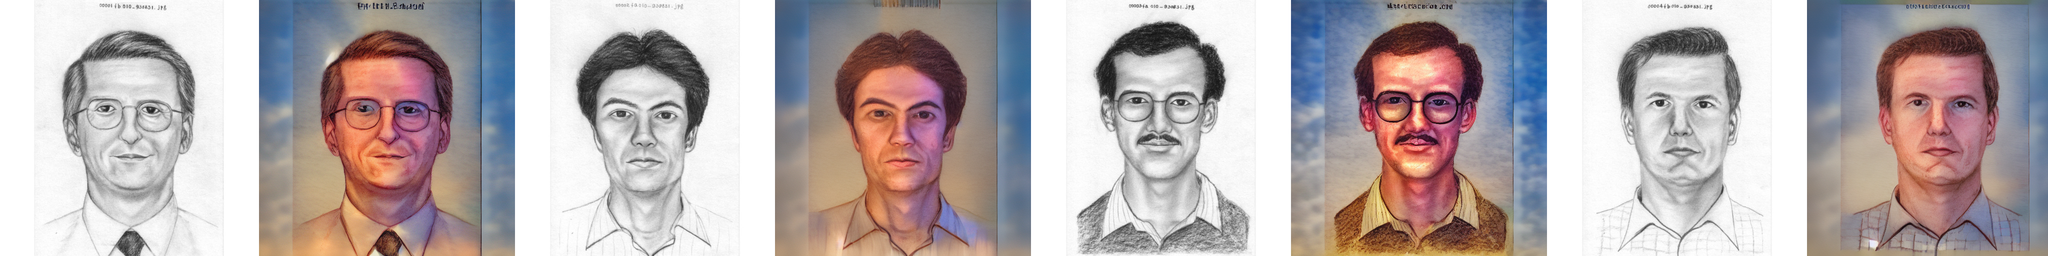
\includegraphics[width=\columnwidth]{figures/sketch}
\caption{손으로 그린 얼굴 스케치(홀수 열)와 모델이 만든 결과(짝수 열), 제로샷.
그림에는 차단 반경이 없으므로 모델이 그림 자체에서 구조 밀도를 읽어야 하며,
조건의 이미지별 최소--최대 정규화가 이를 가능하게 한다.}
\label{fig:sketch}
\end{figure}


그림~\ref{fig:sketch}이 전이 결과다. 학습에 쓰인 적 없는 실제 얼굴 그림
\sketchFaceN{}장에서, 입력 그림에 대한 구조
순응도는 \sketchFaceSC{}, CLIP 점수는 \sketchFaceClip{}이다. FID는 보고하지 않는다.
\sketchFaceN{}장은 안정적인 추정에 부족하고, 평가기가 값을 내는 대신 거부한다.

\section{한계}

쓸 만한 구간은 대략 $r \in [0, 0.3]$이다. 그 위에서는 조건에 남는 에너지가 적어
--- $r{=}0.5$에서 스펙트럼의 0.0014 --- 구조 순응도를 해석하기 어려워진다. 거의
비어 있는 두 신호는 모델이 무엇을 하든 상관이 0에 가깝기 때문이다.

여기 있는 모든 것은 한 도메인(FFHQ 얼굴)과 한 백본(SD1.5)이다. 현재의 구조 제어 연구는
DiT 백본~\cite{peebles2022scalable,esser2024scaling}으로 옮겨갔고, 거기서
LoRA~\cite{hu2021lora} 계열 어댑터~\cite{tan2024ominicontrol,zhang2025easycontrol,liu2025nanocontrol}는
우리보다 훨씬 적은 파라미터로 제어를 보고한다. 우리 효율 수치는 ControlNet 대비로 읽어야 하며 그
연구선과 비교할 것이 아니다.

특화 모델 비교는 정직하지만 $r{=}0.1$에서 불리하고, 사용자 연구는 수행하지 않았다.

\section{결론}

학습 중 구조 조건의 대역폭을 무작위화하면 차단 반경이 추론 시 제어가 되고, 그
제어는 어댑터를 약하게 만드는 것으로 재현되지 않는다. 여기에 도달하려면 조건이
네트워크에 들어가는 위치를 고치고 조건을 냉동 오토인코더 밖에 두어야 했다. 두
발견은 다이얼을 무엇에 쓰든 다른 조건화 설계에도 옮겨간다.

\bibliographystyle{plainnat}
\bibliography{refs}

\end{document}
